%\begin{tikzpicture}
%
%    \def \n {5}
%    \def \radius {3cm}
%    \def \margin {8} % margin in angles, depends on the radius
%    
%    \foreach \s in {1,...,\n}
%    {
%      \node[draw, circle] at ({360/\n * (\s - 1)}:\radius) {$\s$};
%      \draw[->, >=latex] ({360/\n * (\s - 1)+\margin}:\radius) 
%        arc ({360/\n * (\s - 1)+\margin}:{360/\n * (\s)-\margin}:\radius);
%    }
%\end{tikzpicture}

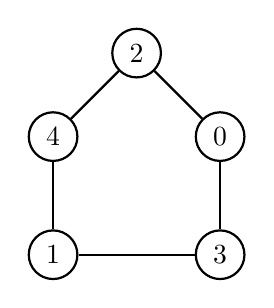
\begin{tikzpicture}[node distance={15mm}, thick, main/.style = {draw, circle}] 
    \node[main] (2) {$2$}; 
    \node[main] (4) [below left of=2] {$4$};
    \node[main] (0) [below right of=2] {$0$};
    \node[main] (1) [below of=4] {$1$};
    \node[main] (3) [below of=0] {$3$};

    \draw (2) -- (4);
    \draw (2) -- (0);
    \draw (4) -- (1);
    \draw (1) -- (3);
    \draw (3) -- (0);
\end{tikzpicture} 